
\chapter{意义位于何处}

\section{什么时候一个事物不总是同样的?}

上一章我们遇见了这样的问题:“什么时候两个事物是同样的?”在这一章,我们要讨论这个问题的反面:“什么时候一个事物不总是同样的?”我们引申出来的论题是:意义是一条消息所固有的,还是在心灵或机器与一条消息的相互作用中产生的——就像在前面的对话中那样?如果是后一种情况,那意义就不能被说成是位于任何一个具体地方,也不能说一条消息有什么普遍的或客观的意义,因为每个观察者都可以把他自己的意义带给每条消息。但如果是前一种情况,那意义既可以被定位,又可以具有普遍性。在本章中我要说明,在某种情况下至少有些消息是具有普遍性的,当然,并不是说所有消息都如此。我们会发现,一条消息有“客观意义”这个想法以一种有趣的方式联系于对智能进行描述时的简单性。

\section{信息携带者与信息揭示者}

我要从我喜爱的例子说起:唱片、音乐和唱机之间的关系。我们对这样的想法感到欣慰:唱片和一段音乐含有同样的信息,因为有可以“阅读”唱片的唱机存在,它可以把槽纹模式转换为声音。换句话说,在槽纹模式和声音之间有一个同构,而唱机是一种以物理方式实现这一同构的机械。这样,可以很自然地把唱片想象成“信息携带者”,而把唱机想象成“信息揭示者”。关于这些概念的另一个例子是由"pq"系统给出的。在那里,“信息携带者”是定理,而“信息揭示者”是解释过程。由于解释是显而易见的,因此我们在从"pq"系统的定理中提取信息时不需要任何电动设备的帮助。

这两个例子给人一种印象:同构和解码机制(即信息揭示者)只不过是在揭示结构中固有的、等着被“抽出来”的信息。这将导致下述想法:在每个结构中都存在着某些能够从中“抽出来”的信息,以及其它一些不能从中抽出来的信息。但所谓“抽出来”到底是什么意思呢?抽的时候允许用多大力气?有些情况下,如果投入足够的努力,你能从特定的结构中抽出非常深奥的信息。实际上,这个抽出过程可能涉及到相当复杂的操作,以致于使你感到你放进去的信息比抽出来的还多。

\section{遗传型和表现型}

以遗传信息为例,它们通常被认为是存在于脱氧核糖核酸(DNA)的双螺旋之中。一个DNA分子——一个“遗传型”——通过一个非常复杂的过程被转化成实在的有机体——一个“表现型”,这个过程包括蛋白质的生成、DNA的复制、细胞的复制、细胞类型的逐渐分化等等。顺便提一下,这种从遗传型到表现型的展开——所谓“渐成过程”——是一种盘根错节的递归,在第十六章中我们将集中讨论这一问题。渐成过程由一组极其复杂的化学循环和带反馈的循环所支配。当整个有机体构成之后,在其机体特征和遗传型之间甚至最微小的相似性也找不到了。

尽管如此,把有机体的机体结构归因于其DNA的结构,而且只归因于它,这已经成了一种标准惯例。这种观点的第一个证据来自于奥斯瓦尔德·艾弗里在1944年所做的实验,从那以后又积累了大量支持这一观点的证据。艾弗里的实验表明,在所有生物分子中,唯有DNA传递了遗传特征。你可以在一个有机体中改变其它分子,例如蛋白质,但这种改变将不会被传递到其后代中去。但是,一旦DNA被改变了,所有后代都将继承这种改变后的DNA。这种实验表明,修改构造新的有机体的指令的唯一途径,是修改DNA——而这又进一步意味着那些指令一定是以某种方式编码于DNA的结构之中的。

\section{异常同构和平凡同构}

因此,人们似乎被迫接受这样的想法:DNA的结构包含了表现型结构的信息,这就是说二者是同构的。但是,这是一种“异常”同构。我这种说法的意思是,要想把表现型和遗传型都分解成能彼此对应的“部分”,这可不是轻而易举就能做到的。与此相对照,在“平凡”同构中,一个结构的各部分可以很容易地对应于另一个结构的各部分。例如唱片和一段音乐之间的同构就是如此,在这种情况下,我们知道对于这段音乐中的任何音响都存在有一个刻在槽纹中的与之精确对应的“像”,而且,如果需要的话,完全可以准确地找到它。平凡同构的另一个例子是G图和其中任何一个“蝴蝶”之间的同构。

在DNA结构与表现型结构之间的同构无论如何也不能算是平凡的,而且实际上完成这一同构的机制复杂得吓人。比如,如果你非要在你的DNA中找出哪一段是关于你鼻子形状或指纹形状的,你的日子一定不会好过。这有点像企图在一段音乐中确定带有某种情感意义的那个音符。显然不存在这样的音符,因为感情意义不是被个别音符,而是被较大的“组块”在高层次上所携带的。附带说一下,这种“组块”并不一定是邻接的音符组成的集合。完全可能是一些不相邻的段落放在一起时带有了某种情感意义。

类似地,“遗传意义”——即关于表现型结构的信息——是遍布于DNA分子的各组成部分之中的,虽然还没有人能懂得这种语言(注意:懂得这种“语言”并不等同于破译遗传密码,要知道,后者在60年代初期就能做到了。遗传密码说明如何把一段段DNA转换成各种氨基酸。因此,破译遗传密码可以类比于弄清某种外语的字母表中各字母的音标,而不包括弄清楚那种语言的语法或单词的意义。在抽取DNA的意义的过程中,遗传密码的破译是必不可少的一步,但这只是漫长的征途中的第一步)。

\section{自动唱机和触发器}

DNA中所包含的遗传意义是隐含意义的最好例子之一。为了将遗传型转换成表现型,必须用一套比遗传型复杂得多的机制作用于遗传型之上。遗传型的各个部分对这套机制起着“触发器”的作用。一台自动唱机——普通的,不是螃蟹的那种!——在这里提供了一个有用的类比:整个机构所要执行的非常复杂的动作由一对按钮来指定,因此那对按钮可以被描述成“触发”了所播放的歌曲。在把遗传型转换成表现型的过程中,“细胞自动唱机”——请你原谅这个概念——从DNA长链的片断中接收了“按钮信号”,而它们所播放的“歌曲”则常常是用来构造新的“自动唱机”的基本元件。这就好像有那么一些真实的自动唱机,它们播放的歌曲的歌词不是赞美爱情的,而是教人如何构造更复杂的自动唱机的……DNA的一部分触发了蛋白质的制造,这些蛋白质触发了千百种新的反应,然后这些反应再去触发复制操作,通过若干步骤对DNA进行复制——如此这般进行下去……从这里可以感觉到这整个过程的递归程度。这个不断触发的过程的最终产物是表现型——个体生物。因而人们说表现型是一开始便潜藏于DNA中的信息的“展现”——或“抽出”(这里用的“展现”这个词来自雅克·莫诺,他是二十世纪最深刻、最有创见的分子生物学家之一)。

现在没有人会说从自动唱机的喇叭里传出的歌声是对唱机按钮中固有信息的“展现”了,那对按钮似乎只是“触发器”,其作用是激活自动唱机中携带信息的那部分。而另一方面,把从唱片中抽取音乐称为对唱片中固有信息的“展现”,这似乎是完全合理的,因为有下面几种理由:
\begin{enumerate}
\item 音乐似乎不是隐藏在唱机的机构之中;
\item 有可能以任意的精确程度把输入(唱片)的片断匹配于输出(音乐)的片断;
\item 有可能在同一台唱机上播放别的唱片,从而得到别的音乐;
\item 唱片和唱机可以很容易地相互分离。
\end{enumerate}

至于一个被打碎的唱片的碎片中是否还包含着固有意义,这完全是另一个问题了。这些碎片可以拼到一起,使原有的信息得以重建——但这里进行着某种更为复杂的过程。继后的问题是关于一个加了密的电话呼叫的固有信息……事实上存在着一系列各种程度的固有意义。你不妨试着在这个系列之中找出渐成过程的位置,这会是很有趣的。当有机体的生长过程发生时,是否可以说信息是从某DNA中“抽出”的?是否关于该有机体结构的全部信息都在那里?

\section{DNA和化学环境的必要性}

从某种意义上说,根据艾弗里等人的试验,对上述问题的回答似乎应该是肯定的。但从另一种意义上说,回答似乎又应是否定的,因为这种抽出过程极大地依赖于非常复杂的细胞化学过程,而这些过程则并非是编码于DNA之中的。DNA所依赖的事实是这些过程将会发生,但它似乎没有包含导致它们发生的任何密码。这样,关于遗传型中的信息的性质,我们就有了两种相互冲突的观点。一种观点认为,既然有这样多的信息在DNA之外,那么把DNA仅仅看成是一套非常复杂的触发装置——就像自动唱机上的一排按钮——是完全合理的。另一种观点则认为,所有信息都已在DNA之中,只不过是以一种极其隐蔽的形式存在而已。

现在看来,这好像只不过是以两种不同的方式说了同一件事。但也未必就是如此。一种观点认为:DNA离开了环境就毫无意义,而另一种观点认为:即使离开了环境,一个来自生物体的DNA分子对其结构来说仍有一种“强制性的内在逻辑”,不管怎样总能推导出它所带的消息。简而言之,一种观点认为:为了使DNA有意义,化学环境是必须的;而另一种观点认为:揭示一束DNA的“固有意义”,只有智能是必须的。

\section{一个假想的飞碟}

为了进一步考察这个问题,让我们考虑一个奇异的假想事件。一张由大卫·奥伊斯特拉赫和列夫·奥博林演奏的巴赫《F小调小提琴钢琴奏鸣曲》的唱片被放在一颗卫星中上了天,然后,它被从卫星中发射出去,走上了离开太阳系,或许离开整个银河系的旅程——一个中间有孔的薄塑料盘,孤零零地旋转着通过星际空间。它当然是离开了它的环境。它能带有多少意义呢?

如果外星人得到了它,他们几乎一定会被它的形状所吸引,而且很可能会对它很感兴趣。这样,它的形状作为一个触发器,立即就带给了他们一些信息:这是一个人工制品,或许还是一个载有信息的人工制品。这个想法——由唱片自身所传送或触发的——这时就创造了一个新的环境,此后这张唱片就将在这个环境中被理解。解码过程的下一步或许需要相当长的时间——那是我们难以估量的。我们可以设想,如果这样的一张唱片在巴赫那个时代到达地球,那么没有人会知道怎么对待它,它很可能得不到释读。但是,这并没有减弱我们的信念:原则上说信息是在那里,只是我们知道那时的人类知识还不够丰富,不足以对付信息在存储、传输和展现过程中的各种可能性。

\section{消息的理解层次}

时至今日,解码这个概念已经被极大地拓广了,成了天文学家、语言学家、考古学家、军事学家等工作中的一个重要组成部分。常常有人提出,我们可能是浮在来自其它文明的无线电信号的汪洋大海中,而这些信号我们还不知道如何释读。已经有许多人在严肃地考虑释读这种信号的技术。主要问题之一——或许是最深刻的问题——是这样的:“我们到底是怎样认出一个信号的存在?也即,怎样确认一个框架?”发送唱片看来是个简单的解决办法——其物理结构的外观很引人注意。至少我们有理由设想,对任何充分进化了的智慧生物来说,它可能触发从中寻找隐藏着的信息的想法。不过,从技术上讲,向其它星系发送固态的物体似乎有些不着边际。虽然如此,也并不妨碍我们考虑这个想法。

我们假设外星人想到了:适用于翻译这张唱片的机制,该是一台能把槽纹转换成声音的机器。这离真正的释读还差得很远。那么,对这样一张唱片的成功释读到底包括些什么呢?显然,这种智慧生物必须能从声音中找到意义。声音本身并无价值,除非这种声音在那种智慧生物的大脑(假如可以这样称呼的话)之中产生预想的触发作用。那么什么是预想的作用呢?就是要在他们的脑中激活某些结构,以产生出类似于我们在听这段曲子时所体验到的那种情感。事实上,甚至可以不通过产生声音,只要他们能以某种别的方式使用唱片来激活他们大脑中的适当结构就行了(如果我们人类能够用别的办法来顺序地触发我们大脑中的适当结构,像音乐所起的作用那样,我们也完全会满足于绕过声音——但是,不用耳朵来接受音乐似乎是极难以想象的。失聪的作曲家——贝多芬、德沃夏克、福莱——或那些看着乐谱就能“听到”音乐的音乐家的存在并不与上述说法相矛盾。他们的这种能力是基于以前数十年的直接听觉体验之上的)。

至此一切都变得复杂了。外星人也有情感吗?如果有的话,是否可能与我们的情感建立起不论何种意义下的对应关系?如果他们确实具有多少与我们相类似的情感,那么这些情感是否也是以多少与我们相同的方式联结在一起的呢?他们是否能理解诸如“悲剧性的美”或“勇敢地忍受”这样的复合概念?如果我们终将发现宇宙中的各种智慧生物在认识结构上与我们是如此相同,以致于情感都是彼此重叠的,那么在某种意义上,这张唱片将永远不会脱离它的自然环境,而这种环境就是事物的自然体系的一部分。如果真是这样的话,一个遨游天际的唱片只要不在途中损坏,最后就很可能被一个或一群外星人得到,并以一种我们会认为是成功的方式释读出来。

\section{“太空幻景”}

前面探讨DNA分子的意义时,我使用了“强制性的内在逻辑”这种说法,而且我认为这是一个关键性的概念。为了说明这一点,让我们略微修改一下那个把唱片送往太空的假想事件,把巴赫的曲子换成约翰·卡奇的《大地幻景第四号》。这支曲子是典型的偶然音乐——其结构是通过各种随机过程选择的,而非致力于传达个人的感受。演奏时,二十四名演奏者操纵着十二台收音机的二十四个旋钮。在乐曲的进行过程中,他们随意转动旋钮,因此每台收音机的声音随机地增大或减少,并不断地变换电台。这样产生的全部音响就构成了这支曲子。卡奇的观点用他自己的话来说,就是“让音响只代表它们自身,而不是作为表达人造理论或人类情感的工具”。

现在设想把这张唱片送入了太空。对外星人来说,理解这件人工制品的本质的可能性简直是微乎其微——如果还不是完全不可能。他们很可能会被框架信息(“我是一条消息,请释读我”)和内部混乱的结构之间的矛盾搞得莫名其妙。在卡奇的这段音乐中,根本没有什么可以凭借的“组块”,也没有什么可以作为释读线索的模式。而另一方面,在巴赫的音乐中似乎有大量可以凭借的东西——模式、模式的模式,如此等等。我们还无从知道这些模式是否在整个宇宙中都能起作用。我们对智能、情感以及音乐的性质了解得还不够,无法断定巴赫音乐的内在逻辑是否在宇宙各处都是有效的,以致于其意义可以跨越星系。

但是,我们在这里要讨论的,不是巴赫的音乐是否具有足够的内在逻辑,而是任何消息是否本质上都具有足够的内在逻辑,一旦遇到具有充分高智能的生物,其环境总能自动地建立起来。如果某些消息确实具有这种重建环境的性质,那么把这段消息的意义看作该消息的固有性质,这似乎就是合理的了。

\section{了不起的释读者}

有助于说明这些想法的另一个例子是古代文字材料的释读,这些材料是由未知的字母组成的未知语言书写的。直觉告诉我们,在这样的文字材料中确有固有信息,不论我们是否能成功地将其展现出来。这是一种很强烈的信念,就像我们虽然一点也不懂阿拉伯文,但仍然相信一张阿拉伯文报纸具有固有的意义。一旦一段文字或语言材料被释读出来,没有人会问其意义是哪里来的:显然是来自于材料,而非释读方法——正如音乐是存在于唱片里,而非唱机中一样!我们鉴别解码机制的办法之一就是根据下列事实:它们不向记号或物体——作为输入的对象——当中添加任何意义,而仅仅是展现出这些记号或物体中的固有意义。一台自动唱机不是一种解码机制,因为它并不展现其输入信号的任何意义,相反,它提供的是隐藏于它自身内部的意义。

古代文献的释读往往需要几组相互竞争的学者花费数十年的劳动,依靠存储在世界各地的图书馆中的知识,才能完成。这种过程也不增加信息吗?当发现解码规则需要这样巨大的努力的时候,意义还在多大程度上是材料所固有的呢?是人把意义赋予了材料,还是意义本来就在那里?我的直觉告诉我,意义从来就在那里。虽然把它抽出来极其费力,但不会抽出原来没在材料中的意义。这个直觉主要来自于一个事实:我觉得释读结果具有必然性。这就是说,即使这段材料不是在这时被这一组人释读出来,那它也一定会被另一组人在另一个时候释读出来——结果将是同样的。这就是意义成为材料本身的一部分的原因所在:它以一种可以预测的方式作用于智能。我们一般可以说:意义在多大程度上以可以预测的方式作用于智能,它就在此程度上是对象的一部分。

\begin{figure}
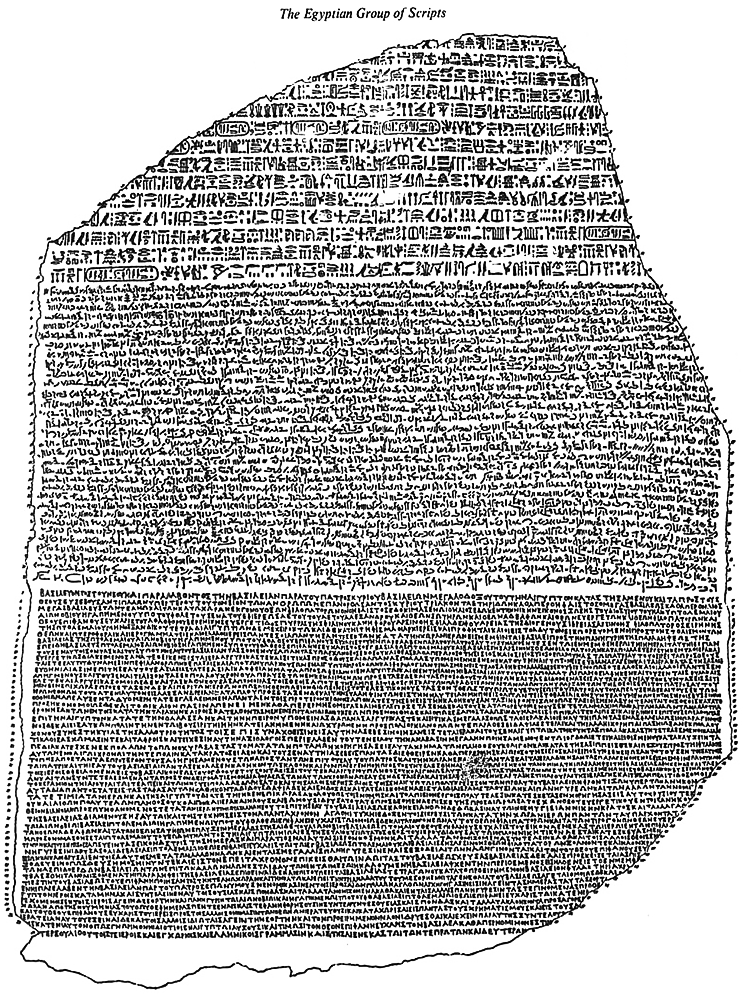
\includegraphics{img_039.png}
\caption{罗塞达碑。}
\end{figure}

\fig{39}表现的是罗塞达碑,它是最珍贵的考古发现之一。它成了释读埃及象形文字的钥匙,因为它载有用三种古文字书写的同一段材料:象形文字、古埃及俗体文字和希腊文字。这段刻在玄武岩石柱上的铭文在1821年首先被有埃及学之父之称的让·弗朗索瓦·尚波里昂所释读。它是聚集在孟菲斯的教士们对托勒密五世表示拥戴的一个决议。

\section{任何消息都分三层}

从这些对脱离环境的消息进行释读的例子中,我们可以清楚地分出信息的三个层面:\pnum{1}框架消息、\pnum{2}外在消息、\pnum{3}内在消息。这当中我们最熟悉的是\pnum{3},即内在消息,它也就是预定要传送的消息:在音乐中是情感体验,在遗传学中是表现型,在书板上是古代文明的王权与礼仪,如此等等。

\begin{block}
理解内在消息就是抽取出发送人所要传递的意义。
\end{block}

框架消息是这样一种消息:“我是一条消息,你有本事就来解译我!”它是由信息携带者总体的结构特征隐含地传递的。

\begin{block}
理解框架消息就是确认需要一种解码机制。
\end{block}

如果确认了这样的框架消息,那么人们的注意力就会转到第2层:外在消息。这是由消息中符号的模式及结构隐含地携带的信息,说明如何去解译内在消息。

\begin{block}
理解外在消息就是建造——或知道如何建造——能正确解译内在消息的解码机制。
\end{block}

这个外在层次必然是一种隐含消息,就是说发送者无法肯定它是否会被理解。试图发送一些说明如何解译外在消息的指示,那注定是徒劳的。因为这些指示必然是内在消息的一部分,所以只有当发现了解码机制之后才能被理解。由于这个缘故,外在消息就必须是一组触发器,而不是那种由已知解码器去揭示的消息。

为分析意义是如何包含在消息之中的,上述三个“层次”的划分只不过是一个很粗糙的初级阶段。在外在和内在消息之中可能有许多层,而不是只有一层。作为一个例子,让我们考虑一下罗塞达碑的内在和外在消息是怎样错综复杂地相互缠绕的。一段消息的彻底释读,有赖于重建支持这一消息的产生的整个语义结构——从而在每一个深入的方面理解消息发送者。这样我们完全可以把内在消息抛开不管,因为如果我们真的理解了外在消息的所有精妙之处,内在消息也就能重新构造出来了。

乔治·斯坦纳的著作《巴别塔之后》对内在消息和外在消息之间的相互作用进行了长篇讨论(虽然他没有使用这两个术语)。这本书的韵味可以从下面的引文中体现出来:

\begin{quote}
我们经常会使用速写式的办法,而其背后蕴藏着丰富的潜意识以及故意隐瞒着或故意暴露着的联想,它们非常广泛和复杂,差不多构成了我们作为一个个体的全部独特之处。\note{乔治·斯坦纳,《告别巴别塔之后》,第172--173页。}
\end{quote}
列奥纳德·迈尔在他的著作《音乐、美术与思想》中也表达了类似的想法:

\begin{quote}欣赏埃利奥特·卡特的曲子的方式完全不同于那种恰当地倾听约翰·卡奇的曲子的方式。类似地,阅读贝克特的小说的方式也必须在很大程度上区别于读贝娄的小说。而对威廉·德·库宁的绘画和安迪·瓦豪尔的绘画也需要不同的感知认识态度。\note{列奥纳德·迈尔,《音乐、美术与思想》,第87--88页。}
\end{quote}

对于艺术作品来说,努力传递风格也许是最为重要的,在这种情况下,如果你彻底把握了一种风格,你也就不再需要那种风格的作品了。“风格”、“外在消息”、“解码技术”——所有这些都不过是表达同一个基本观念的不同方式而已。

\section{薛定谔的非周期性晶体结构}

是什么东西使我们在某些对象中看到框架消息,而在另一些对象中则看不到呢?当外星人截获了一张在太空中漂游的唱片时,他们凭什么假定其中隐含着消息?一张唱片和一块陨石有什么不同?显然,其几何形状提供了最初的线索,说明“这是些有趣的东西”。下一条线索是,在微观尺度上,它是由一条很长的非周期性的模式序列构成,这一序列绕成了一条螺线。假如我们把这条螺线展开,就会得到一条极长的由微小的符号组成的线性序列(约2000英尺)。这很像一个DNA分子,后者的符号是从只包含四种不同的碱基的“字母表”中选取的,这些符号排成一维序列,然后绕成一个螺旋。在艾弗里建立基因和DNA的联系之前,物理学家欧文·薛定谔在他有影响的著作《生命是什么?》中作出了纯理论预言,认为遗传信息一定是存储于“非周期性晶体结构”之中。事实上,书籍本身就是规整的几何形状中的非周期性晶体结构。这些例子说明,一旦我们在某处发现一个非常规则的几何结构中“包裹着”非周期性晶体结构,那里就可能隐藏着一些内在消息(我不是说这就是框架消息的全部特征,但是,事实上许多常见消息的框架消息都满足这一描述。\fig{40}中有许多说明问题的例子)。作为局外人,当我在思索意义是怎样隐藏在这些美丽的非周期性晶体结构的奇妙曲线与折角之中时,我深深地沉浸在一种神秘的气氛里。形式里就存在着内容。

\begin{figure}
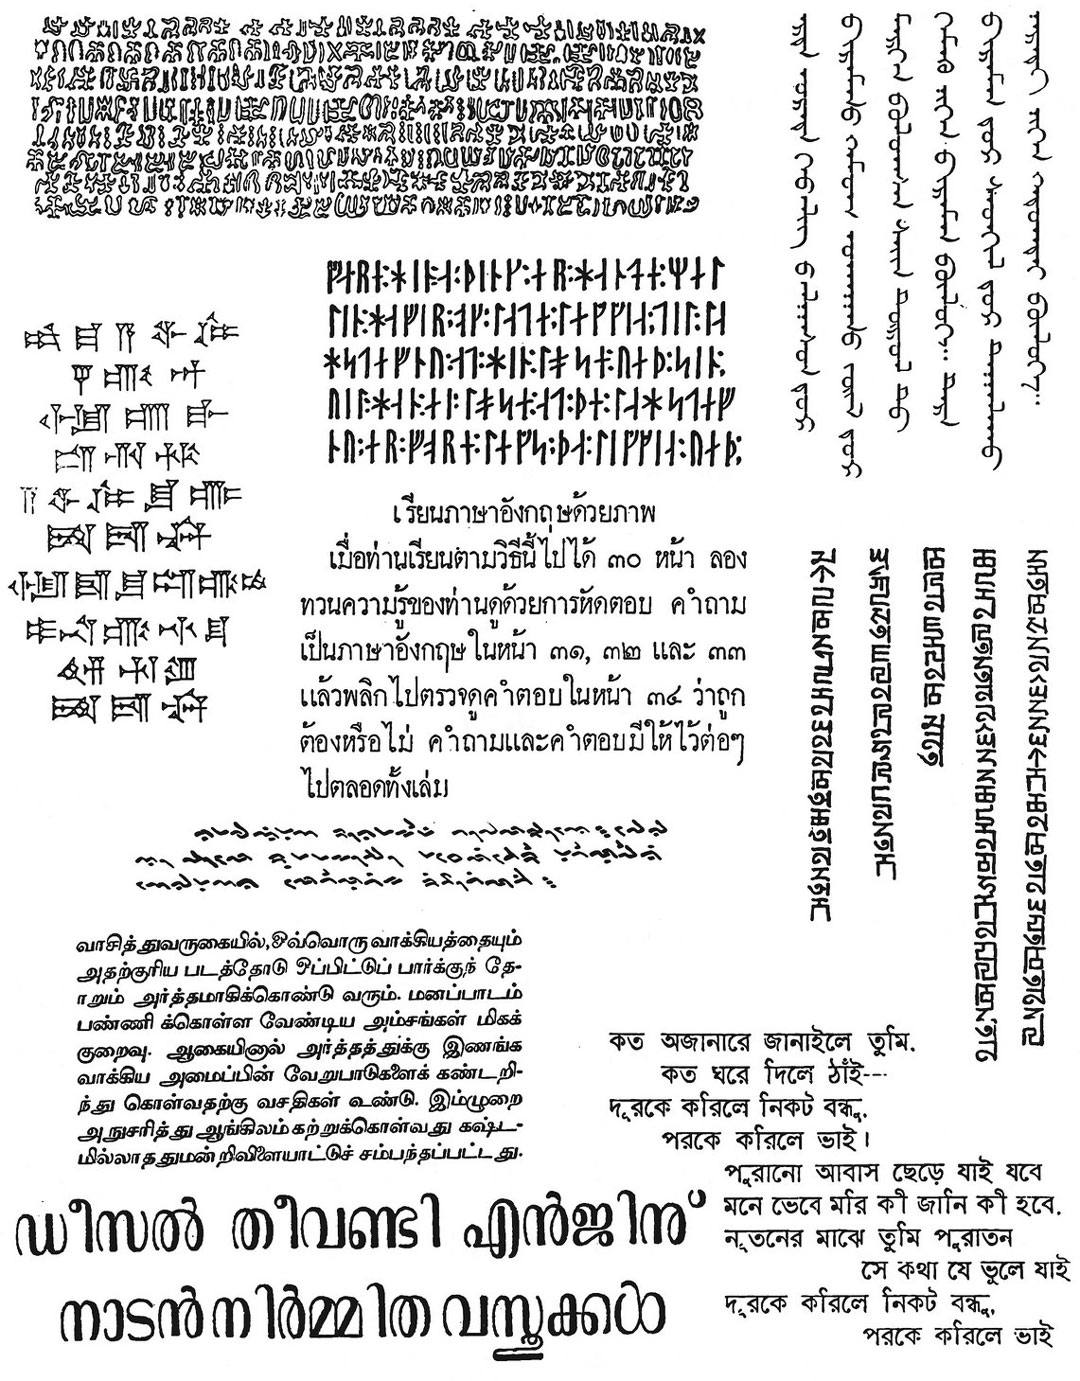
\includegraphics[height=.7\textheight]{img_040.jpg}
\caption{文字集。}
\floatfoot{左上角是一段尚未释读的铭文,发现于复活节岛。它是用“犁耕体”写的,即奇数行从左向右读,偶数行从右向左读。字符刻在一块$35$英寸长,$4$英寸宽的木制书板上。顺时针方向的下一个是竖写的蒙文:上面是现代蒙文,下面是写于1314年的一段公文。再往下,在右下角我们见到的是一段用孟加拉文写的诗,作者是拉宾德拉那特·泰戈尔。它的左边是一条马莱亚拉姆文(使用于印度南部的西喀拉拉)的报纸标题。往上看是一段曲线优美的泰米尔文(使用于东喀拉拉)。再往上的一小段摘自一个布金文(使用于印度尼西亚的西勒伯斯岛)的民间故事。在字体集的中央是一段泰文。它的上方是一段写于十四世纪的古北欧文手稿,其中记载着斯堪尼亚(瑞典南部)地方法律的一个案例。最后,一段古代亚述国的楔形文字挤在了左边,它是汉谟拉比法典中的一节。\note{引自汉斯·詹森[Hans Jensen],《记号、符号与字体》[\bn{Sign, Symbol, and Script}],(纽约:G.Putnam's Sons,1969年版),89页(楔形文字),356页(复活节岛),386页、417页(蒙文),552页(古北欧文);肯尼思·卡兹纳[Kenneth Katzner],《世界的语言》[\bn{The Languages of the World}],(纽约:Funk and Wagnalls,1975年版),190页(盂加拉文),237页(布金文);里查兹和克里斯廷·吉布森[I. A. Richards and Christine Gibson],《英语图解》[\bn{English Through Pictures}],(纽约:Washington Square Press,1960年版),73页(泰米尔文),82页(泰文)。}}
\end{figure}

\section{三个层次上的语言}

对于从海滩上的瓶子里发现的消息来说,信息三个层次是很清楚的。一旦某个人拾到了它,看出它是海上漂来的,并见到里面装着一张干燥的纸条,他就会发现第一个层次,即框架消息。甚至在没看到字迹的情况下,他也能认识到这种人工制品是一个信息携带者。这时候扔下瓶子不看个究竟,只可能是那种异乎寻常地麻木不仁的人才干得出来。这么做几乎可以说是缺乏人性的。紧接着,他会打开瓶子,并查看纸条上的记号。或许上面是用日文写的,发现这一点并不需要对其内在消息有任何理解——只要能认出字母就够了。这种外在消息写成中文就是“我是用日文写的”。一旦发现了这一点,这个人就能进入内在消息,那可能是遇难者的呼救,也可能是一首小诗,或是一封情书……

把“这条消息是用日文写的”翻译成日文后放在内在消息中,那是无济于事的——如果有人要阅读它首先就得懂得日文。他在阅读这段消息之前,首先必须认识到,由于这是日文,所以自己能读懂它。你可能会想到把“这条消息是用日文写的”翻译成许多种不同的文字写在这张纸上,以此来摆脱困境。实用上这是有意义的,但从理论上看困难依然如故。一个懂汉语的人仍然必须先看出这条消息的“汉语性”,否则于事无补。因此,一个无法回避的难题是,必须从外部发现如何释读内在消息。虽然内在消息本身也可以提供线索和证据,但这些最多也不过是作用于发现瓶子的人(或他所求助的人)的触发器而已。

收听短波广播的人面临着类似的难题。首先,他必须确定他所听到的声音是否确实构成了一条消息,是否只不过是静电干扰。声音本身并不能对此作出回答,即使是在下述可能性极小的情况下也是如此:内在消息就是用收听者本人的母语构成的,说的是“这些声音确实构成了一条消息,而不仅仅是静电干扰!”如果收听者在这些声音中识别出了框架消息,然后他就会设法辨认广播所使用的语言——显然,这时他依然在外面。他从广播中接收到了触发器,但它们并没有把答案明确地告诉他。

外在消息的本性就决定了它们不可能被任何显式的语言所传达。试图发现一种能够传达外在消息的显式语言将不会有任何进展——因为这种想法本身在概念上就已经自相矛盾了。理解外在消息对于收听者来说永远是责无旁贷的。如果成功,他就能进入消息的内部,这时触发器和显现出的意义之间的比率将大幅度移向后者。和前几个阶段相比,内在消息的理解似乎是水到渠成的事,就像是自动冒出来的一样。

\section{意义的“自动唱机”理论}

这些例子看起来似乎是支持了这样一个观点:没有什么消息是具有固有意义的,原因是不论要理解哪种内在消息,哪怕它再简单,也必须首先理解其框架消息和外在消息,而这两者是只由触发器所传递的(例如由日文字母写成,或具有螺线型沟槽等)。那么,这好像开始意味着我们无法摆脱关于意义的一种“自动唱机”理论——这种观点认为:消息不包含固有意义,因为在任何消息被理解之前,它都会被用作某个“自动唱机”的输入,而这就意味着该“自动唱机”所包含的信息一定会在消息中的意义被获取之前加在它上面。

这个论点很像在刘易斯·卡罗尔的对话中乌龟为阿基里斯设置的那个圈套。在对话中,这个圈套表现为下述想法:在你能使用任何规则之前,你必须有另一个规则来告诉你如何使用这一规则;换句话说,存在一个具有无穷多层次的规则体系,这就阻止了任何规则的使用。在我们这里,这个圈套表现为下述想法:在你理解任何一条消息之前,你必须有另一条消息来告诉你如何理解这条消息;换句话说,存在一个具有无穷多层次的消息体系,这就阻止了对任何消息的理解。但是,我们都知道这些悖论是无效的,因为规则的确是在被使用,而消息也的确是在被理解。这是怎么回事呢?

\section{反驳自动唱机理论}

这是因为,我们的智能并未“出窍”,而是表现于我们的大脑这种物理对象之中。我们大脑的结构是漫长的进化过程的结果,它们的运行是受物理规律控制的。既然它们是物理实体,我们的大脑在运行时无需被告知如何运行。就是在这一层次上,物理规律产生出思维,因而卡罗尔的规则悖论被打破了。与此相类似,在大脑把输入数据解释成消息的那个层次上,消息悖论被打破了。似乎大脑原本就配备着一些“硬件”来识别哪些东西是消息,而且能对这些消息进行解码。就是这种最低限度的抽取内在意义的天生能力使得高度递归的、滚雪球式的语言习得过程得以发生。这种天生的硬件就像一台自动唱机:它提供一些附加信息,把那些触发信号转换成完整的消息。

\section{若智能是自然的,则意义是固有的}

如果不同的人的“自动唱机”里的“歌曲”是不同的,而且它们都以各自不同的方式反应于给定的触发信号,那么我们就不会倾向于把意义作为触发信号所固有的东西。但是,人类大脑的构造导致如下情形:在同样条件下,一个脑和另一个脑对一个给定的触发信号几乎产生完全一样的反应。这就是一个幼儿能够学会一门语言的原因,他对触发信号的反应方式和其他幼儿相同。这种“人类自动唱机”的统一性就造成了一种统一的“语言”,这种语言可用来交流框架消息和外在消息。进一步说,如果我们相信人类智能只不过是一种普遍存在的自然现象的一个特例——即智能生物会出现于各种各样的环境之中——那么可以推测,人们用来交流框架消息和外在消息的“语言”只不过是智能生物彼此之间进行通讯的那种通用语言的一种“方言”而已。这样,有几种触发信号该是具有“普遍触发能力”的,就是说,所有智能生物都趋向于以和我们同样的方式对这些触发信号作出反应。

这就使我们得以改变关于意义位何处的叙述。我们可以把一条消息的意义(框架的、外在的、内在的)归因于消息自身,因为事实上释读机制本身是具有普遍性的——这就是说,它们是自然界的基本形式,以同样的方式产生于形形色色的环境之中。具体来说,假设“A-5”键在所有自动唱机上都触发同样的歌——同时进一步假设自动唱机不是人工制品,而是一种普遍存在的自然对象,就像星系或碳原子那样。在这种情况下,我们或许会赞同把“A-5”的普适触发能力称为它的“固有意义”,而且,“A-5”会得到“消息”的头衔,而不再叫“触发器”,同时,那首歌会确实成为“A-5”的固有意义的一种“展现”,虽然这种意义是以隐含方式存在的。

\section{地球沙文主义}

把意义归因于消息是出于这样一种看法:分布在宇宙各处的智能生物对消息所进行的处理具有不变性。这有点像把质量归因于物体。对于古代人来说,似乎一个物体的重量一定是该物体的固有属性。但当人们懂得了引力之后,人们认识到重量取决于物体所处的引力场。然而,一个相关的量,即质量,却是不随引力场的变化而变化的。从这种不变性中人们得出了结论:一个物体的质量才是物体自身的一种固有属性。如果将来发现质量也是随环境而变的,那我们会回过头来重新修正我们关于物体固有属性的观点。根据同样的道理,我们可以设想,或许存在着其它种类的“自动唱机”——其它种类的智能生物——他们之间相互通讯所用的消息是我们所无法识别的,同样他们也无法把我们的消息认作是消息。如果事实果真如此,那么认为意义是一组符号的固有属性的观点将需要重新考虑。不过,我们又怎么可能发现这种生物的存在呢?

把这种“固有意义”的论点与那种与此平行的“固有重量”的论点相比较将是很有趣的。假设某人把一个物体的重量定义为“当此物体处于行星地球的表面时产生的向下方的力的量度”。在这个定义下,当一个物体处于火星表面时,它产生的向下方的力就不能被称为“重量”,而要另找个词。按这个定义,重量成了一种固有属性,但其代价是地球中心观——“地球沙文主义”。这有点像“格林威治沙文主义”——即拒绝承认地球上除格林威治平时之外的其它地区时间。这样看待时间未免太古怪了。

也许我们在智能问题上已经不自觉地背上了类似的沙文主义包袱,导致在意义问题上也是这样。在我们的沙文主义观点下,我们可能把那些具有和我们充分相似的大脑的生物称为“智能生物”,同时拒绝承认其它类型的东西是具有智能的。举一个极端的例子:设想有一块陨石,它没有去释读那张游荡在太空的巴赫唱片,而是在相遇时对唱片完全置之不理,只管走自己的路。在我们看来,它和唱片的相互作用方式不涉及唱片的意义。因此,我们会倾向于认为它是“愚钝的”。但我们这样做很可能是错怪了这块陨石。也许它正是具有一种“更高级的智能”,是我们这些带着地球沙文主义眼光的人所无法感知到的。而它与唱片的相互作用恰恰是这种高级智能的表现。那么,也许唱片也具有一种“更高级的意义”——完全不同于我们所赋予它的那种意义。也许它的意义取决于接收它的智能的类型。也许。

如果我们不说“有智能就表现为在一串符号中取出的消息和我们所取出的一样”,而以某种别的方式来定义智能,那将是令人高兴的。因为如果我们只能以这一种方式来定义,那我们对于意义是一种固有属性的论证就是循环论证,因此是毫无内容的。我们应当设法以某种独立的方式来确定“智能”这个名称所应具有的一组特征。这些特征应当能构成人所共有的智能的统一核心。在历史的现阶段,我们还没有得到这些特征的一张清楚的表。但是,看来在近几十年中对人类智能的认识很可能得到长足的进展。尤其是认知心理学家、人工智能研究人员和神经学家,他们或许能综合他们的理解,以导致一个对智能的定义。这个定义可能仍然是人类沙文主义的,我们无法摆脱这一点。但作为一种补偿,可能会有某种雅致、漂亮——而且可能十分简单——的抽象方式来定义智能的本质特征。这将有助于减弱我们那种由于得到了一个以人类为中心的概念而产生的不安。当然,如果我们与其它星系的外星人建立了联系,那就会支持我们的这种信念:我们所具有的这种智慧不仅仅是一种侥幸,而是反复再现于自然界的各种环境中的一种基本形态之中的一例,就像星星和铀原子核一样。这反过来又会支持意义是一种固有属性的观点。

为了结束这个论题,让我们考虑一些新旧例子,并讨论它们具有固有意义的程度。我们要采取的方式是:使我们尽可能地置身于一个截获了神秘物体的外星人的立场……

\section{太空中的两块金属板}

设想有一块金、银、铜的合金板,在上面刻着两个点,一个在另一个之上:就像这个冒号的样子。虽然这个物体的整体形状暗示了它是一个人工制品,因此可能隐藏着某种消息,但只有两个点尚不足以说明任何问题。(在读下去之前,你能猜出它们可能意味着什么吗?)但假设我们造出了第二块板,上面有更多的点,像下图这样:
\begin{center}
\def~{\ \textcdot \ }
~\\
~\\
~~\\
~~~\\
~~~~~\\
~~~~~~~~\\
~~~~~~~~~~~~~\\
~~~~~~~~~~~~~~~~~~~~~\\
~~~~~~~~~~~~~~~~~~~~~~~~~~~~~~~~~~
\end{center}

现在显然应当做的——起码对地球上的智慧生物来说是如此——就是依次去数一下每行中有多少个点,结果会得到这样一个序列:
\[
  1, 1, 2, 3, 5, 8, 13, 21, 34
\]
在这里有证据证明从一行推到下一行是被一条规则所控制的。事实上,从这个序列中可以有把握地推断出斐波那契数定义的递归部分。假设我们把开始的一对数值$(1,1)$当作“遗传型”,用一条递归规则就可以从中推出“表现型”——整个斐波那契序列。如果只向太空送出遗传型——即第一块金属板——那我们还没能送出使表现型得以重建的信息。因此,遗传型并没有包含对表现型的完整说明。但另一方面,如果我们把第二块金属板当作遗传型,那么将有比较充足的理由设想表现型确实会被重建。这种新的遗传型——可称之为“长遗传型”——所包含的信息足以使智能生物能够仅从遗传型中推出把表现型从遗传型中抽取出来所需要的机制。

一旦这种从遗传型中抽取表现型的机制得以稳固地建立,我们就能回过头来使用“短遗传型”——例如第一块板。比如说“短遗传型”$(1,3)$将导出下面的表现型:
\[
  1, 3, 4, 7, 11, 18, 29, 47, \dotsc
\]
——这就是卢卡斯序列。对任意一对初始值——即对每种短遗传型——来说,都存在一个对应的表现型,但短遗传型不同于长遗传型,它们只起触发器的作用——就像自动唱机上的按钮,而递归规则是建立在自动唱机内部的。长遗传型包含有充足的信息,能够对智能生物进行触发,使他们知道该建造什么样的“自动唱机”。在这种意义下,长遗传型包含了关于表现型的信息,而短遗传型则没有。换句话说,长遗传型不仅传送了内在消息,而且传送了外在消息,这就使内在消息得以被读出。看起来外在消息的明确性取决于消息的长度。这并不出人意料,因为这完全类似于释读古代文献时的情况。显然,释读成功的可能性极大程度上取决于所占有的文献数量。

\section{再谈巴赫之别于卡奇}

但仅有很长的材料还是不够的。让我们再看看把巴赫和约翰·卡奇的音乐唱片送入太空时,两者之间的差异。首先让我们看看卡奇的曲子对我们有什么意义。卡奇的曲子必须被放在巨大的文化背景中去考察——作为对某种传统观念的反叛。这样,如果我们想传送这种意义,我们必须不仅传送曲子中的音符,而且还必须事先传送详尽的西方文化史。这恐怕意味着一张孤立的约翰·卡奇音乐唱片是没有固有意义的。但是,对一个精通东西方文化,尤其是熟知西方音乐在近几十年中的发展趋势的听众来说,这张唱片确实具有某种意义——可这样的听众则像一台自动唱机了,而曲子像一对按钮。意义在开始时已经几乎都在他的头脑里,音乐只不过是起了触发的作用而已。这种“自动唱机”与纯粹智能不同,它们完全不具有普遍性。它们仅限于地球,依赖于一个相当长的时期内全球事件的特定序列。希望外星人能理解卡奇的音乐,就好像希望你所喜欢的一首曲子在月亮上的一台自动唱机上的按钮号码和在南美的一个酒店里的一台自动唱机上的按钮号码是一样的。

在另一方面,要欣赏巴赫的曲子就远不需要那样多的文化知识。这真像是一种极大的讽剌,因为巴赫是如此复杂而又有条理,卡奇则是极端地缺乏理智。但这里出现了一个奇怪的颠倒:智能喜爱模式化,厌恶随机性。对大多数人来说,需要对卡奇音乐中的随机性进行大量解释。即便是在解释之后,他们仍会觉得找不到消息——而对巴赫的多数作品来说,解释完全是多余的。在那种情况下,巴赫的音乐和卡奇的音乐相比具有较高的自足性。但我们仍不清楚能听懂巴赫音乐的人必须具有哪些条件。

例如,音乐有三个主要的结构维度(旋律、和声、节奏),每个又可分别由一些小范围的、中间的或者总体的侧面组成。对这些因素中的任何一个,大脑所能直接把握的复杂性都是在一定限度之内的。显然,作曲家在进行音乐创作时往往不自觉地考虑了这一点。这些关于不同因素的“可容忍的复杂程度”,很可能很大程度上依赖于我们人类物种进化的某些特定条件,而其他智慧生物所发展的音乐,在这些因素的可容忍复杂程度上,可能会与我们完全不同。因此可以想象,在传送巴赫的曲子时可能要伴随传送许多关于人类的信息,这些信息是无法仅从音乐的结构中推导出来的。如果我们把巴赫的音乐看成遗传型,把它想要激发出来的情感看成表现型,那么我们所感兴趣的问题是遗传型是否包含了表现型的展现过程所需要的全部信息。

\section{DNA中的消息有多大普遍性?}

我们面临着一个带有一般性的问题,它与那两块金属板所引发的问题相类似,就是:“若要恢复一条消息,需要在多大程度上理解它所处的环境?”我们至此可以回到“遗传型”和“表现型”本来的生物学意义之上——即DNA和活的有机物——来问类似的问题。DNA是否具有普遍的触发能力?或者说它是否需要一台“生物自动唱机”来展示它的意义?DNA在没有被置入适当的化学环境时是否仍能导出表现型?对这个问题的回答是否定的,但是这是一种有限制的否定。当然,真空中的一个DNA分子是什么也创造不出来的。但是,如果把一个DNA分子送到宇宙中去碰碰运气,就像我们设想中的巴赫和卡奇的唱片一样,那它就有可能被外星人所截获。他们可能会首先识别出它的框架消息。如果成功,他们接下去可能设法从它的化学结构推测它所需要的化学环境,然后去提供这样一个环境。沿着这样的途径,通过一些更精细的尝试,终将导致完整地恢复展示DNA的表现型意义所需要的化学环境。这听起来有点像天方夜谭,但如果允许进行亿万年的实验,或许DNA的意义最终还是会显现出来的。

另一方面,如果构成一条DNA的碱基序列是以抽象符号的形式(如\fig{41})被送出,而不是作为长长的螺旋形分子被送出,那么,用这种外在消息来触发那种能把表现型从遗传型中抽取出来的解码机制,其成功的可能性实质上是零。在这种情况下用来包裹内在消息的外在消息实在是太抽象了,它已经失去了恢复环境的能力,因此在实用的意义上来说,这组符号是不具有固有意义的。为了不使你觉得上述讨论过分抽象化和哲学化,请想一下下面这个当今在某些国家高度敏感的问题:到底在哪个时刻才能说遗传型已经“达到”或“隐含”了表现型?这也就是堕胎的合法性问题。

\begin{figure}
%\includegraphics{img_041.png}
\begin{dnaseq}
CCGTCAGGATTGACACCCTCCCAATTGTATGTTTTCATGCCTCCAAATCTTGGAGGCTTTTTTATGGTTCGT
TCTTATTACCCTTCTGAATGTCACGCTGATTATTTTGACTTTGAGCGTATCGAGGCTCTTAAACCTGCTATT
GAGGCTTGTGGCATTTCTACTCTTTCTCAATCCCCAATGCTTGGCTTCCATAAGCAGATGGATAACCGCATC
AAGCTCTTGGAAGAGATTCTGTCTTTTCGTATGCAGCCCGTTGAGTTCGATAATGGTGATATGTATGTTGAC
GGCCATAAGGCTGCTTCTGACGTTCGTGATGAGTTTGTATCTGTTACTGAGAAGTTAATGGATGAATTGGCA
CAATGCTACAATGTGCTCCCCCAACTTGATATTAATAACACTATAGACCACCGCCCCGAAGGGGACGAAAAA
TGGTTTTTAGAGAACGAGAAGACGGTTACGCAGTTTTGCCGCAAGCTGGCTGCTGAACGCCCTCTTAAGGAT
ATTCGCGATGAGTATAATAACCCCAAAAAGAAAGGTATTAAGGATGAGTGTTCAAGATTGCTGGAGGCCTCC
ACTAAGATATCGCGTAGAGGCTTTGCTATTCAGCGTTTGATGAATGCAATGCGACAGGCTCATGCTGATGGT
TGGTTTATCGTTTTTGACACTCTCACGTTGGCTGACGACCGATTAGAGGCGTTTTATGATAATCCCAATGCT
TTGCGTGACTATTTTCGTGATATTGGTCGTATGGTTCTTGCTGCCGAGGGTCGCAAGGCTAATGATTCACAC
GCCGACTCCTATCAGTATTTTTGTGTGCCTGAGTATGGTACAGCTAATGGCCGTCTTCATTTCCATGCGGTG
CACTTTATGCGGACACTTCCTACAGGTAGCGTTGACCCTAATTTTGGTCGTCGGATACGCAATCGCCGCCAG
TTAAATAGCTTGCAAAATACGTGGCCTTATGGTTACAGTATGCCCATCCCAGTTCGCTACACGCAGGACGCT
TTTTCACCTTCTGGTTGGTTGTGGCCTGTTGATGCTAAAGGTGAGCCGCTTAAAGCTACCAGTTATATGGCT
GTTGGTTTCTATGTGCCTAAATACGTTAACAAAAAGTCAGATATGGACCTTGCTGCTAAAGGTCTAGGAGCT
AAAGAATGGAACAACTCACTAAAAACCAAGCTGTCGCTACTTCCCAAGAAGCTGTTCAGAATCAGAATGAGC
CGCAACTTCGGGATGAAAATGCTCACAATGACAAATCTGTCCACGGAGTGCTTAATCCAACTTACCAAGCTG
GGTTACGACGCGACGCCGTTCAACCAGATATTGAAGCAGAACGCAAAAAGAGAGATGAGATTGAGGCTGGGA
AAAGTTACTGTAGCCGACGTTTTGGCGGCGCAACCTGTGACGACAAATCTGCTCAAATTTATGCGCGCTTCG
ATAAAAATGATTGGCGTATCCAACCTGCAGAGTTTTATCGCTTCCATGACGCAGAAGTTAACACTTTCGGAT
ATTTCTGATGAGTCGAAAAATTATCTTGATAAAGCAGGAATTACTACTGCTTGTTTACGAATTAAATCGAAG
TGGACTGCTGGCGGAAAATGAGAAAATTCGACCTATCCTTGCGCAGCTCGAGAAGCTCTTACTTTGCGACCT
TTCGCCATCAACTAACGATTCTGTCAAAAACTGACGCGTTGGATGAGGAGAAGTGGCTTAATATGCTTGGCA
CGTTCGTCAAGGACTGGTTTAGATATGAGTCACATTTTGTTCATGGTAGAGATTCTCTTGTTGACATTTTAA
AAGAGCGTGGATTACTATCTGAGTCCGATGCTGTTCAACCACTAATAGGTAAGAAATCATGAGTCAAGTTAC
CGAACAATCCGTACGTTTCCAGACCGCTTTGGCCTCTATTAAGCTCATTCAGGGTTCTGCCGTTTTGGATTT
AACCGAAGATGATTTCGATTTTCTGACGAGTAACAAAGTTTGGATTGCTACTGACCGCTCTCGTGCTCGTCG
CTGCGTTGAGGCTTGCGTTTATGGTACGCTGGACTTTGTAGGATACCCTCGCTTTCCTGCTCCTGTTGAGTT
TATTGCTGCCGTCATTGCTTATTATGTTCATCCCGTCAACATTCAAACGGCCTGTCTCATCATGGAAGGCGC
TGAATTTACGGAAAACATTATTAATGGCGTCGAGCGTCCGGTTAAAGCCGCTGAATTGTTCGCGTTTACCTT
GCGTGTACGCGCAGGAAACACTGACGTTCTTACTGACGCAGAAGAAAACGTGCGTCAAAAATTACGTGCGGA
AGGAGTGATGTAATGTCTAAAGGTAAAAAACGTTCTGGCGCTCGCCCTGGTCGTCCGCAGCCGTTGCGAGGT
ACTAAAGGCAAGCGTAAAGGCGCTCGTCTTTGGTATGTAGGTGGTCAACAATTTTAATTGCAGGGGCTTCGG
CCCCTTACTTGAGGATAAATTATGTCTAATATTCAAACTGGCGCCGAGCGTATGCCGCATGACCTTTCCCAT
CTTGGCTTCCTTGCTGGTCAGATTGGTCGTCTTATTACCATTTCAACTACTCCGGTTATCGCTGGCGACTCC
TTCGAGATGGACGCCGTTGGCGCTCTCCGTCTTTCTCCATTGCGTCGTGGCCTTGCTATTGACTCTACTGTA
GACATTTTTACTTTTTATGTCCCTCATCGTCACGTTTATGGTGAACAGTGGATTAAGTTCATGAAGGATGGT
GTTAATGCCACTCCTCTCCCGACTGTTAACACTACTGGTTATATTGACCATGCCGCTTTTCTTGGCACGATT
AACCCTGATACCAATAAAATCCCTAAGCATTTGTTTCAGGGTTATTTGAATATCTATAACAACTATTTTAAA
GCGCCGTGGATGCCTGACCGTACCGAGGCTAACCCTAATGAGCTTAATCAAGATGATGCTCGTTATGGTTTC
CGTTGCTGCCATCTCAAAAACATTTGGACTGCTCCGCTTCCTCCTGAGACTGAGCTTTCTCGCCAAATGACG
ACTTCTACCACATCTATTGACATTATGGGTCTGCAAGCTGCTTATGCTAATTTGCATACTGACCAAGAACGT
GATTACTTCATGCAGCGTTACCATGATGTTATTTCTTCATTTGGAGGTAAAACCTCATATGACGCTGACAAC
CGTCCTTTACTTGTCATGCGCTCTAATCTCTGGGCATCTGGCTATGATGTTGATGGAACTGACCAAACGTCG
TTAGGCCAGTTTTCTGGTCGTGTTCAACAGACCTATAAACATTCTGTGCCGCGTTTCTTTGTTCCTGAGCAT
GGCACTATGTTTACTCTTGCGCTTGTTCGTTTTCCGCCTACTGCGACTAAAGAGATTCAGTACCTTAACGCT
AAAGGTGCTTTGACTTATACCGATATTGCTGGCGACCCTGTTTTGTATGGCAACTTGCCGCCGCGTGAAATT
TCTATGAAGGATGTTTTCCGTTCTGGTGATTCGTCTAAGAAGTTTAAGATTGCTGAGGGTCAGTGGTATCGT
TATGCGCCTTCGTATGTTTCTCCTGCTTATCACCTTCTTGAAGGCTTCCCATTCATTCAGGAACCGCCTTCT
GGTGATTTGCAAGAACGCGTACTTATTCGCAACCATGATTATGACCAGTGTTTCAGTCGTTCAGTTGTTGCA
GTGGATAGTCTTACCTCATGTGACGTTTATCGCAATCTGCCGACCACTCGCGATTCAATCATGACTTCGTGA
TAAAAGATTGAGTGTGAGGTTATAACCGAAGCGGTAAAAATTTTAATTTTTGCCGCTGAGGGGTTGACCAAG
CGAAGCGCGGTAGGTTTTCTGCTTAGGAGTTTAATCATGTTTCAGACTTTTATTTCTCGCCACAATTCAAAC
TTTTTTTCTGATAAGCTGGTTCTCACTTCTGTTACTCCAGCTTCTTCGGCACCTGTTTTACAGACACCTAAA
GCTACATCGTCAACGTTATATTTTGATAGTTTGACGGTTAATGCTGGTAATGGTGGTTTTCTTCATTGCATT
CAGATGGATACATCTGTCAACGCCGCTAATCAGGTTGTTTCAGTTGGTGCTGATATTGCTTTTGATGCCGAC
CCTAAATTTTTTGCCTGTTTGGTTCGCTTTGAGTCTTCTTCGGTTCCGACTACCCTCCCGACTGCCTATGAT
GTTTATCCTTTGGATGGTCGCCATGATGGTGGTTATTATACCGTCAAGGACTGTGTGACTATTGACGTCCTT
CCCCGTACGCCCGGCAATAACGTCTACGTTGGTTTCATGGTTTGGTCTAACTTTACCGCTACTAAATGCCGC
GGATTGGTTTCGCTGAATCAGGTTATTAAAGAGATTATTTGTCTCCAGCCACTTAAGTGAGGTGATTTATGT
TTGGTGCTATTGCTGGCGGTATTGCTTCTGCTCTTGCTGGTGGCGCCATGTCTAAATTGTTTGGAGGCGGTC
AAAAAGCCGCCTCCGGTGGCATTCAAGGTGATGTGCTTGCTACCGATAACAATACTGTAGGCATGGGTGATG
CTGGTATTAAATCTGCCATTCAAGGCTCTAATGTTCCTAACCCTGATGAGGCCGCCCCTAGTTTTGTTTCTG
GTGCTATGGCTAAAGCTGGTAAAGGACTTCTTGAAGGTACGTTGCAGGCTGGCACTTCTGCCGTTTCTGATA
AGTTGCTTGATTTGGTTGGACTTGGTGGCAAGTCTGCCGCTGATAAAGGAAAGGATACTCGTGATTATCTTG
CTGCTGCATTTCCTGAGCTTAATGCTTGGGAGCGTGCTGGTGCTGATGCTTCCTCTGCTGGTATGGTTGACG
CCGGATTTGAGAATCAAAAAGAGCTTACTAAAATGCAACTGGACAATCAGAAAGAGATTGCCGAGATGCAAA
ATGAGACTCAAAAAGAGATTGCTGCCATTCAGTCGGCGACTTCACGCCAGAATACGAAAGACCAGGTATATG
CACAAAATGAGATGCTTGCTTATCAACAGAAGGAGTCTACTGCTCGCGTTGCGTCTATTATGGAAAACACCA
ATCTTTCCAAGCAACAGCAGGTTTCCGAGATTATGCGCCAAATGCTTACTCAAGCTCAAACGGCTGGTCAGT
ATTTTACCAATGACCAAATCAAAGAAATGACTCGCAAGGTTAGTGCTGAGGTTGACTTAGTTCATCAGCAAA
CGCAGAATCAGCGGTATGGCTCTTCTCATATTGGCGCTACTGCAAAGGATATTTCTAATGTCGTCACTGATG
CTGCTTCTGGTGTGGTTGATATTTTTCATGGTATTGATAAAGCTGTTGCCGATACTTGGAACAATTTCTGGA
AAGACGGTAAAGCTGATGGTATTGGCTCTAATTTGTCTAGGAAATAA
\end{dnaseq}
\caption[噬菌体$\varphi\mathrm{X}174$染色体的碱基序列。]
  {这个巨大的非周期性晶体结构是噬菌体$\varphi\mathrm{X}174$染色体的碱基序列。它是所有生物中第一个被完整地给出的染色体组。如果要展示争个大肠杆菌细胞的碱基序列,就需要用人约$2000$页纸来写这种犁耕体。展示单个人体细胞DNA的碱基序列大约需要一百万页纸。现在你手中这本节所包含的信息量差小多等于描写一个渺小的大肠杆菌细胞的结构的信息量。}
\end{figure}
